\section{Appendix}

\begin{table}[h]
\centering
\captionsetup{singlelinecheck=false, justification=centering}
\caption{Summary statistics for nominal and real rates (annualized rates) \\ \cite{collard11} sample (1960:I to 2006:IV)}
\label{implied-vs-ffr-nipa-collard}
\begin{tabular}{lccccc} \hline
& Data & SEP & SEP + HP & NSEP & NSEP + HP \\ \hline
\multicolumn{6}{c}{Real interest rates} \\ \hline
\csvreader[head to column names, late after line = \\]%
  {tables/nipa-collard-real.csv}{}%
  {\stat & \data & \sep & \sephp & \nsep & \nsephp} \hline
\multicolumn{6}{c}{Nominal interest rates} \\ \hline
\csvreader[head to column names, late after line = \\]%
  {tables/nipa-collard-nominal.csv}{}%
  {\stat & \data & \sep & \sephp & \nsep & \nsephp} \hline
\end{tabular}
\end{table}

\begin{figure}[h]
\ContinuedFloat*
\centering
\captionsetup{singlelinecheck=false, justification=centering}
\caption{SEP + HP implied vs. observed rates \\ Left: real rates, $\rho = -0.050$. Right: nominal rates, $\rho = 0.142$.}
\label{implied-vs-ffr-nipa-others}
\begin{tabular}{cc}
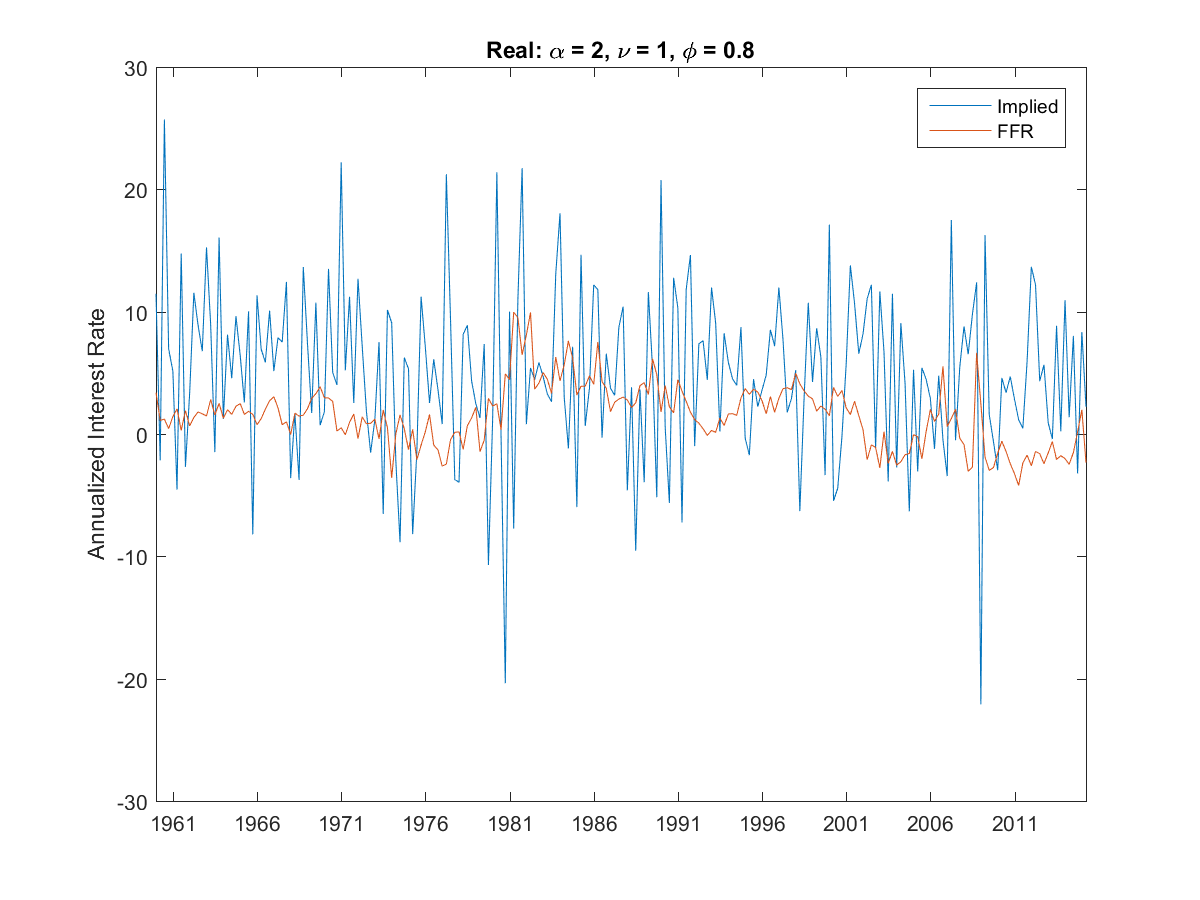
\includegraphics[width=0.5\textwidth]{figs/nipa/real_sep-hp} &
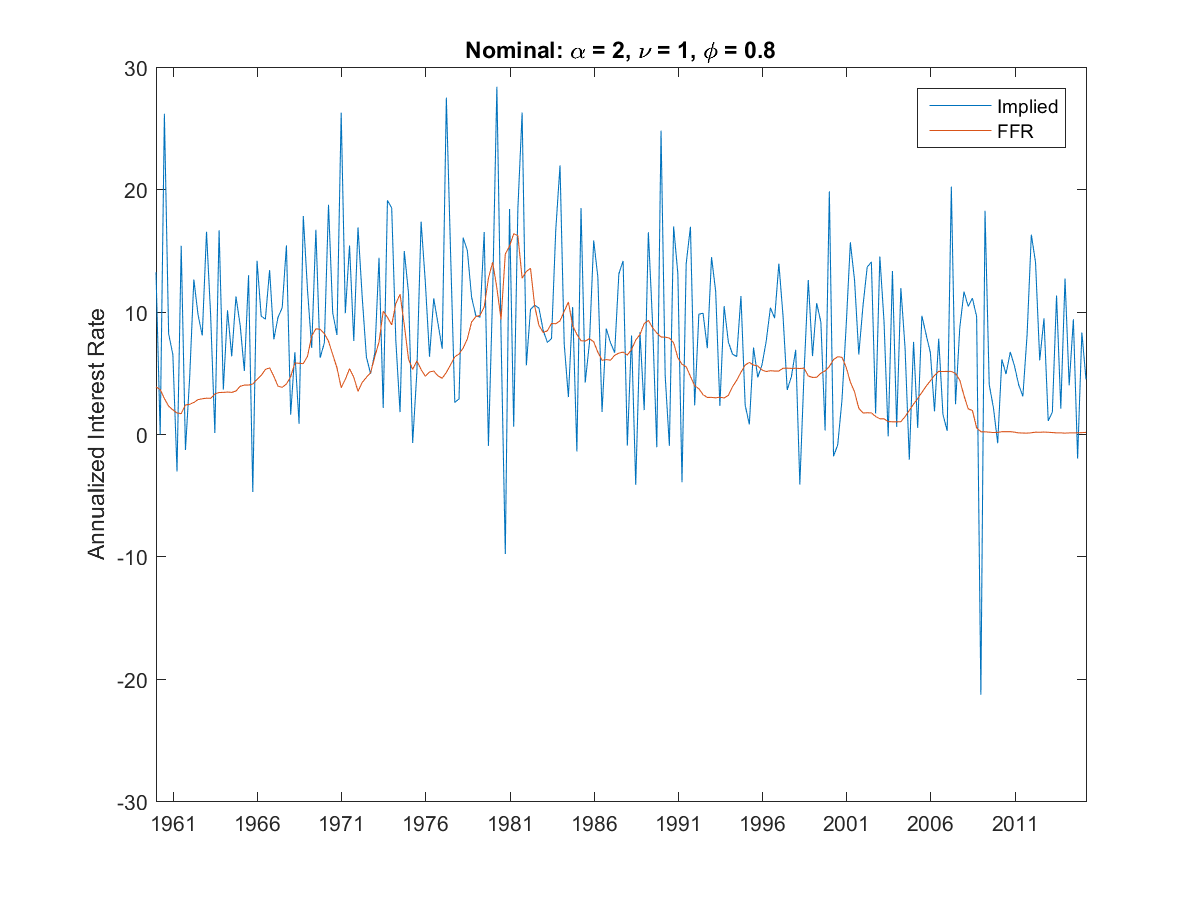
\includegraphics[width=0.5\textwidth]{figs/nipa/nominal_sep-hp}
\end{tabular}
\end{figure}

\begin{figure}[h]
\ContinuedFloat
\centering
\captionsetup{singlelinecheck=false, justification=centering}
\caption{NSEP  implied vs. observed rates \\ Left: real rates, $\rho = 0.261$. Right: nominal rates, $\rho = 0.707$.}
\begin{tabular}{cc}
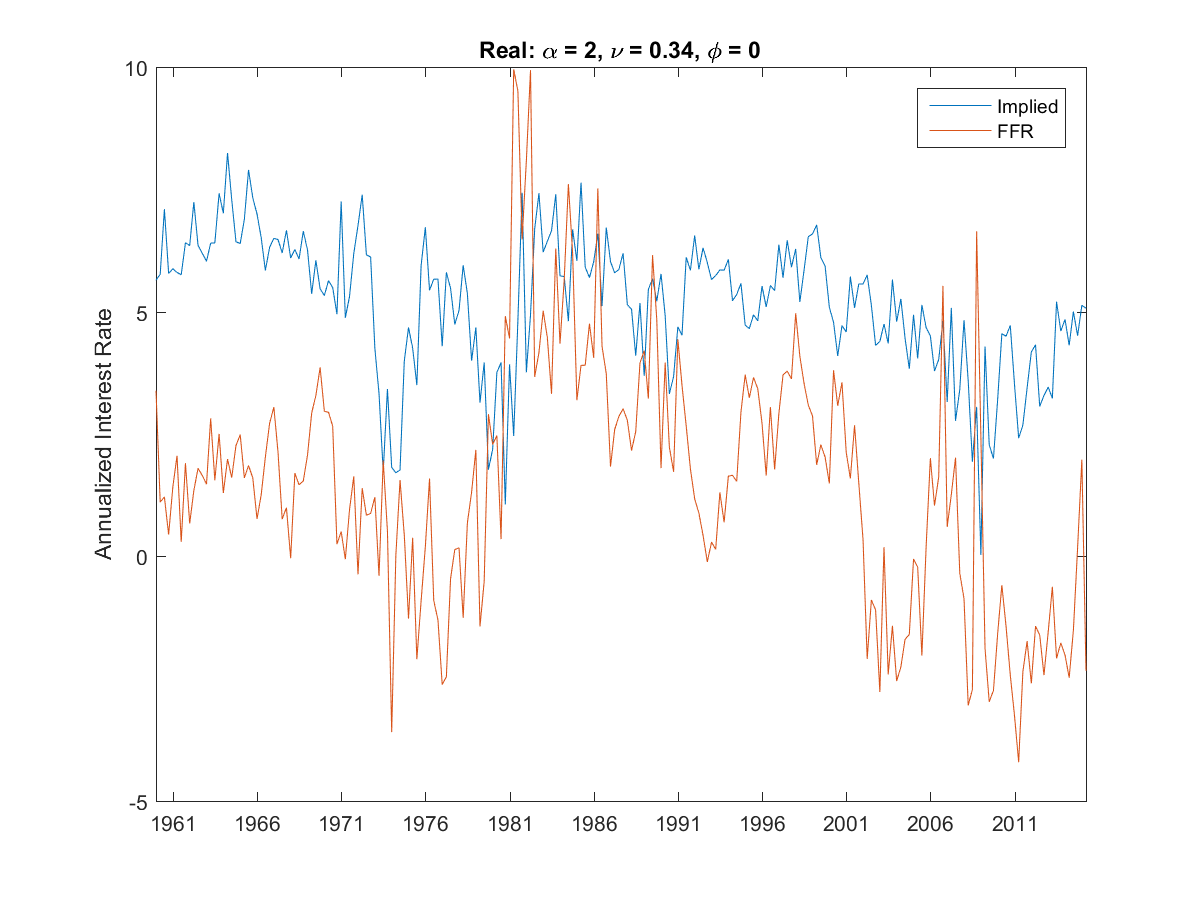
\includegraphics[width=0.5\textwidth]{figs/nipa/real_nsep} &
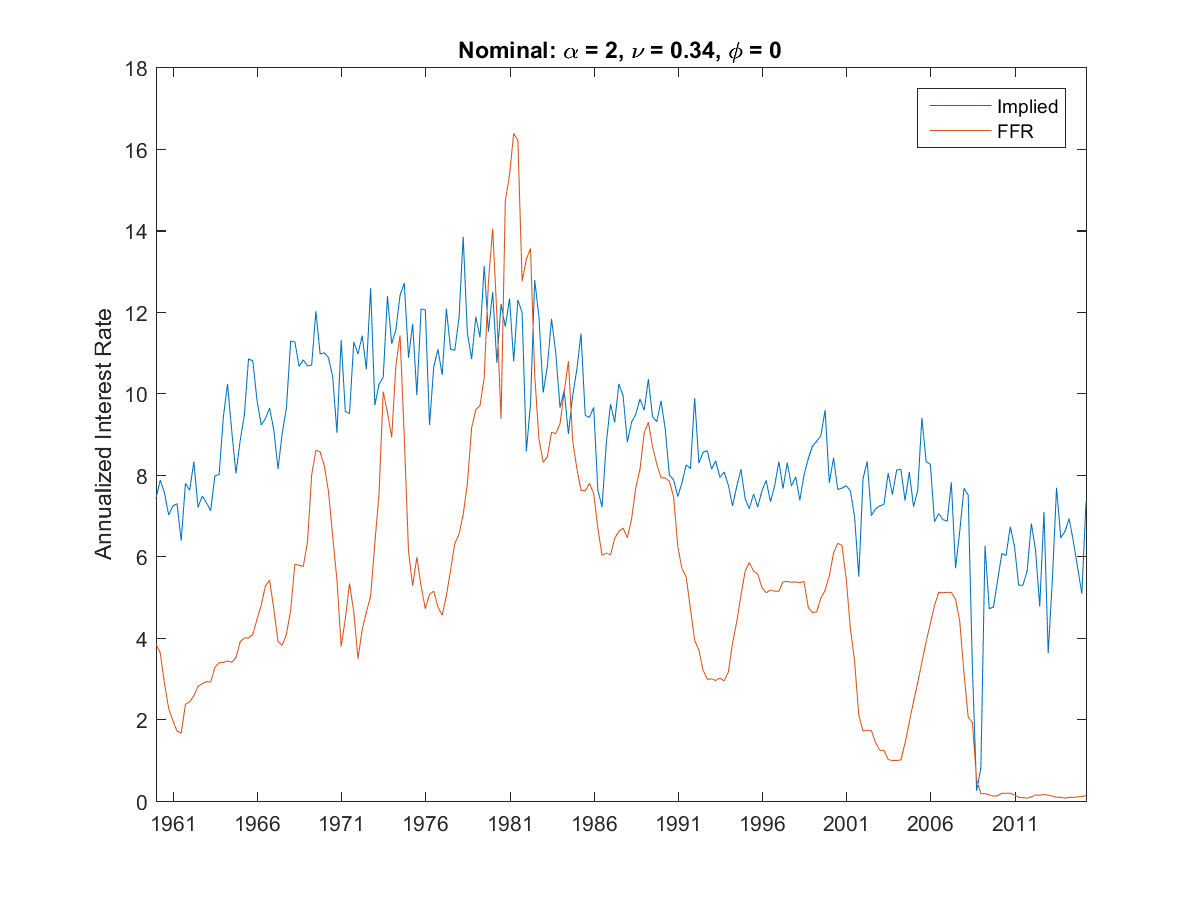
\includegraphics[width=0.5\textwidth]{figs/nipa/nominal_nsep}
\end{tabular}
\end{figure}

\begin{figure}[h]
\ContinuedFloat
\centering
\captionsetup{singlelinecheck=false, justification=centering}
\caption{NSEP + HP implied vs. observed rates \\ Left: real rates, $\rho = 0.033$. Right: nominal rates, $\rho = 0.390$.}
\begin{tabular}{cc}
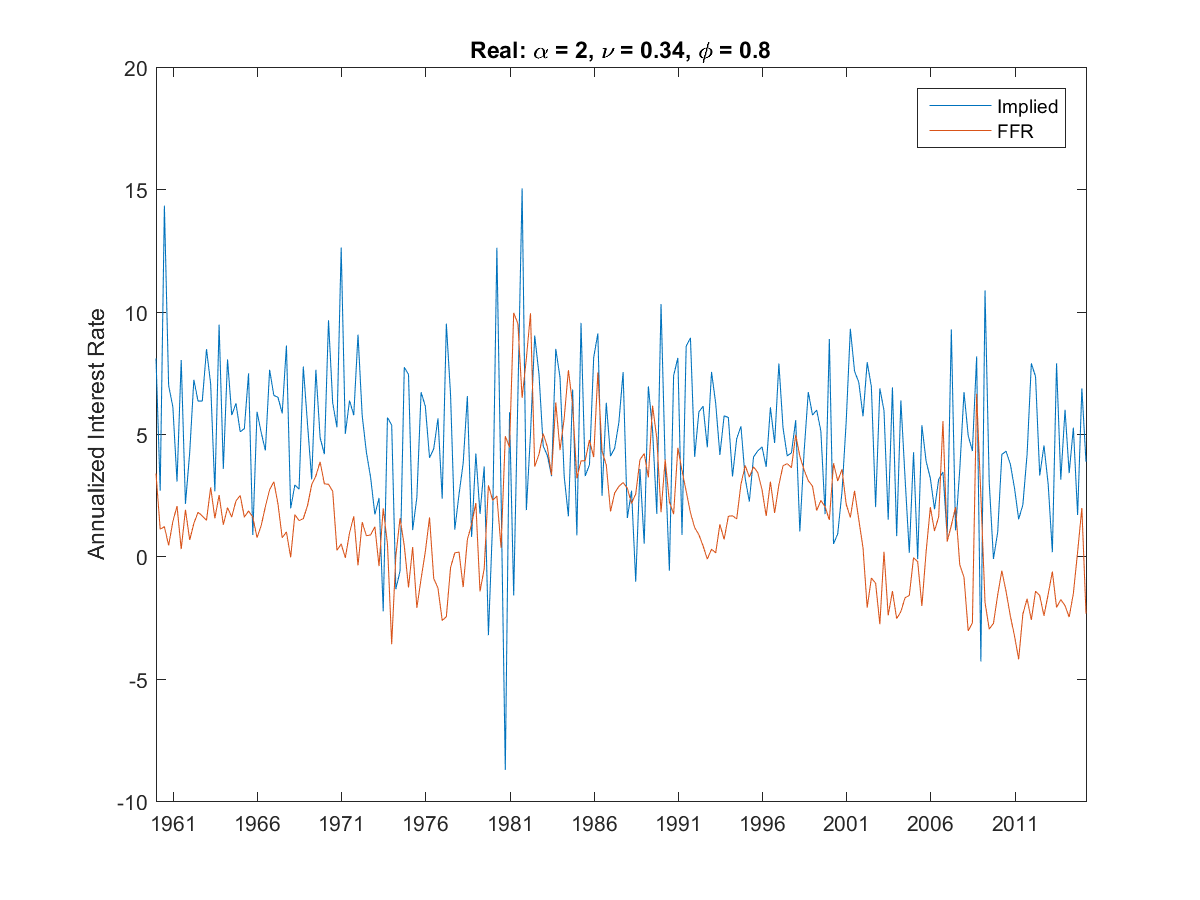
\includegraphics[width=0.5\textwidth]{figs/nipa/real_nsep-hp} &
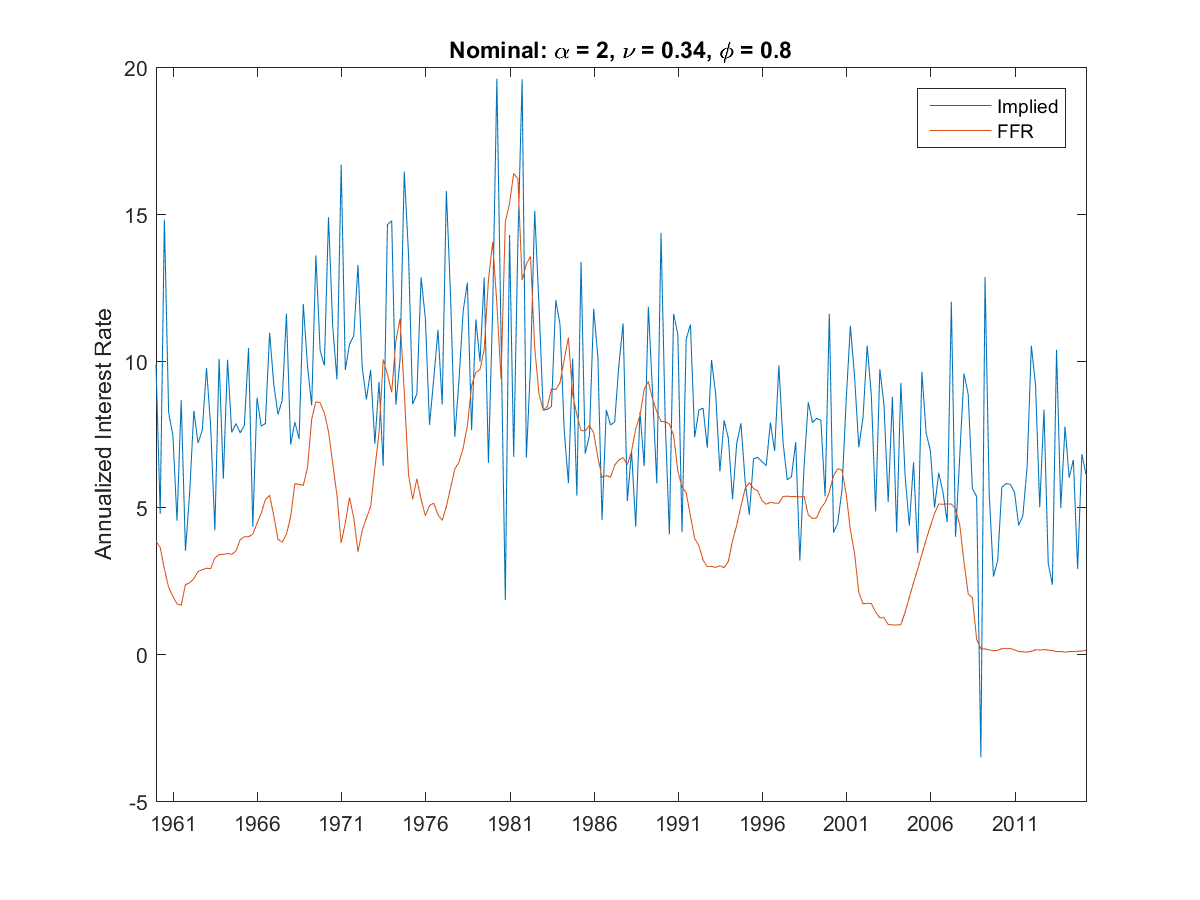
\includegraphics[width=0.5\textwidth]{figs/nipa/nominal_nsep-hp}
\end{tabular}
\end{figure}